%%
%% This is file `sample-acmlarge.tex',
%% generated with the docstrip utility.
%%
%% The original source files were:
%%
%% samples.dtx  (with options: `acmlarge')
%% 
%% IMPORTANT NOTICE:
%% 
%% For the copyright see the source file.
%% 
%% Any modified versions of this file must be renamed
%% with new filenames distinct from sample-acmlarge.tex.
%% 
%% For distribution of the original source see the terms
%% for copying and modification in the file samples.dtx.
%% 
%% This generated file may be distributed as long as the
%% original source files, as listed above, are part of the
%% same distribution. (The sources need not necessarily be
%% in the same archive or directory.)
%%
%%
%% Commands for TeXCount
%TC:macro \cite [option:text,text]
%TC:macro \citep [option:text,text]
%TC:macro \citet [option:text,text]
%TC:envir table 0 1
%TC:envir table* 0 1
%TC:envir tabular [ignore] word
%TC:envir displaymath 0 word
%TC:envir math 0 word
%TC:envir comment 0 0
%%
%%
%% The first command in your LaTeX source must be the \documentclass command.
\documentclass[acmlarge]{acmart}

\usepackage{color}
\usepackage{listings}
\lstset{language=Go,
  basicstyle=\ttfamily\scriptsize,
  keywordstyle=\color{blue}\ttfamily,
  stringstyle=\color{red}\ttfamily,
  commentstyle=\color{green}\ttfamily}
\AtBeginDocument{%
  \providecommand\BibTeX{{%
    \normalfont B\kern-0.5em{\scshape i\kern-0.25em b}\kern-0.8em\TeX}}}

\setcopyright{acmcopyright}
\copyrightyear{2022}
\acmYear{2022}
\acmDOI{}


%%
%% These commands are for a JOURNAL article.
\acmJournal{POMACS}
\acmVolume{37}
\acmNumber{4}
\acmArticle{1}
\acmMonth{8}

\begin{document}
\title{Paper Reading of \textit{Time, Clocks, and the Ordering of Events in a Distributed System}}

%%
%% The "author" command and its associated commands are used to define
%% the authors and their affiliations.
%% Of note is the shared affiliation of the first two authors, and the
%% "authornote" and "authornotemark" commands
%% used to denote shared contribution to the research.
\author{Yiwei Yang}
\email{yangyw@shanghaitech.edu.cn}
\orcid{0000-0001-8011-5868}
\affiliation{
  \institution{ShanghaiTech University}
  \streetaddress{1 R.D. Zhongke}
  \city{Shanghai}
  \state{Shanghai}
  \country{China}
  \postcode{21210}
}
\renewcommand{\shortauthors}{Yiwei Yang}

%%
%% The abstract is a short summary of the work to be presented in the
%% article.
\begin{abstract}
  The paper \cite{lamport2019time} presents a fundamental concept for the ordering of an event in a distributed system.
  And once we have the formal definition of ordering, how we can use it to solve synchronization
  problems. Happens before, or partial ordering of events without precise physical time in the system
  is the assurance of Lamport Clock to be defined. In distributed mutual exclusion, they must release
  granted resources before can be granted again, they should grant resources in order they are made, and
  every request should be eventually granted, assuming the process will not fail. A naive remedy of
  Lamport Clock's opposite is a vector clock to store all nodes' time as a vector. Eventually, it formally defined physical clocks
  with distributed implementation. Based on that, the example of Network Time Protocol is introduced.
\end{abstract}

%%  
%% The code below is generated by the tool at http://dl.acm.org/ccs.cfm.
%% Please copy and paste the code instead of the example below.
%%
\begin{CCSXML}
  <ccs2012>
  <concept>
  <concept_id>10010520.10010553.10010562</concept_id>
  <concept_desc>Distributed System~Lamport Clocks</concept_desc>
  <concept_significance>500</concept_significance>
  </concept>
  <concept>
  <concept_id>10010520.10010575.10010755</concept_id>
  <concept_desc>Vector Clocks~Physical Clocks</concept_desc>
  <concept_significance>300</concept_significance>
  </concept>
  </ccs2012>
\end{CCSXML}

\ccsdesc[500]{Distributed System~Lamport clocks}
\ccsdesc[500]{Distributed System~Network Time Protocol}

%%
%% Keywords. The author(s) should pick words that accurately describe
%% the work being presented. Separate the keywords with commas.
\keywords{distributed system, Lamport clock, sequential consistency, NTP}


%%
%% This command processes the author and affiliation and title
%% information and builds the first part of the formatted document.
\maketitle

\section{Strong Point of the paper}


\subsection {The author defined \texttt{Ordering} and \texttt{Clock}}
\subsubsection{\texttt{Total Ordering} and \texttt{Partial Ordering}}
The author specify the sequential consistency (every core sees same read or write order),
and Release consistency (every core sees write in unlock order)
Happened before, which is the partial consistency, means the small relation satisfying:
\begin{itemize}
  \item Either one event on the same process is ordered.
  \item Message ordered after associated message sends.
  \item As shown in the left graph down below, we can conclude the
        transitivity that $a \rightarrow b$ and $b \rightarrow c$ implies $a \rightarrow c$
\end{itemize}

We can write the state in go using structs and message is to maintain the process id and the type whether is Ack or Processing,
and time is the logical time:

\begin{lstlisting}

  type LamportLockState struct {                  type Message struct {
    time int                                      	Type int // Message type
    proc int                                      	Proc int // Origin process
    seen     []int                                	Time int // Logical time on origin
    channels []chan Message                       }
    reqs     *MessageHeap                         
    lock sync.Mutex                               type MessageHeap []Message
  }                 
  \end{lstlisting}


\begin{figure}[h]
  \centering
  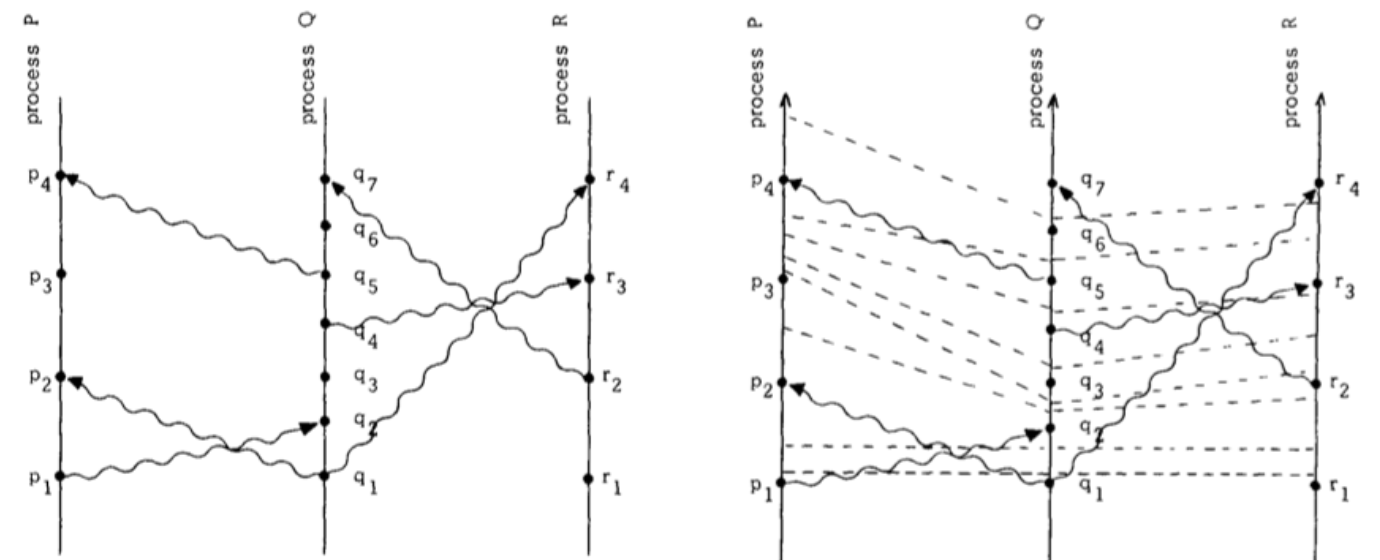
\includegraphics[width=\linewidth]{partial_order.png}
  \caption{Partial ordering of events in the system. Vertical bars are processes.
    Wavy arrows are messages. A dot is an event. Time elapses bottom up.}
\end{figure}

The definition of happened before actually break the convention that the
system must have physical clocks every node for keeping precise physical
time which may have clock skewing problems.

\subsubsection{Logical(Lamport) Clocks}
The logical clocks can be simply defined by clock condition:
\begin{itemize}
  \item if $a \rightarrow b$ then Clock $(a)<\operatorname{Clock}(b)$.
  \item If $a$ is the sending of a message by process $P_{i}$ and $b$ is the receipt
        of that message by process $P_{j}$ then Clo ${ }_{i}(a)<\operatorname{Clock}_{j}(b)$
\end{itemize}
By the dotted line, the condition assures the transmission of timestamp data should appear and across between concrete lines. One possible
implementation using this timestamp is:

\begin{itemize}
  \item \textbf{C1} Each process $P_{i}$ increments $C_{i}$ between any two successive events
  \item \textbf{C2} \begin{itemize}
          \item Send $T_{m}=C_{i}(a)$ along with the message from $a$.
          \item Upon receiving that message, $P_{j}$ sets its $C_{j}$ to be $\geq$ its present value and $>T_{m}$
        \end{itemize}
\end{itemize}

In Go implementation:

\begin{lstlisting}
func (state *LamportLockState) processMessage(m Message) {        } else if m.Type == MessageRelease {       
  // update the process-time vector and current time <- C2          // release previous request       
  state.seen[m.Proc] = m.Time                                       kept := make([]Message, 0)               
  if m.Time > state.time {                                          for state.reqs.Len() > 0 {             
    state.time = m.Time                                              req := heap.Pop(state.reqs).(Message)         
  }                                                                   if req.Proc != m.Proc {                           
                                                                      kept = append(kept, req) 
  // if needed (i.e. not just a MessageAck), update request heap      }       }      
  if m.Type == MessageRequest {                                     for _, req := range kept 
    // new request: add to queue                                     {                      
    heap.Push(state.reqs, m)                                          heap.Push(state.reqs, req)                   
    // reply with an acknowledgement <- C1                          }                                     
    state.sendAckMsg(m.Proc)                                      }
                                                                 }      
  \end{lstlisting}

In Lamport's system of logical clocks if $a \rightarrow b$ then $C(a)<C(b)$. However, the opposite is not true for
\begin{itemize}
  \item if $C(a)<C(b)$, it is not necessarily true that $a \rightarrow b$
        \begin{figure}[h]
          \centering
          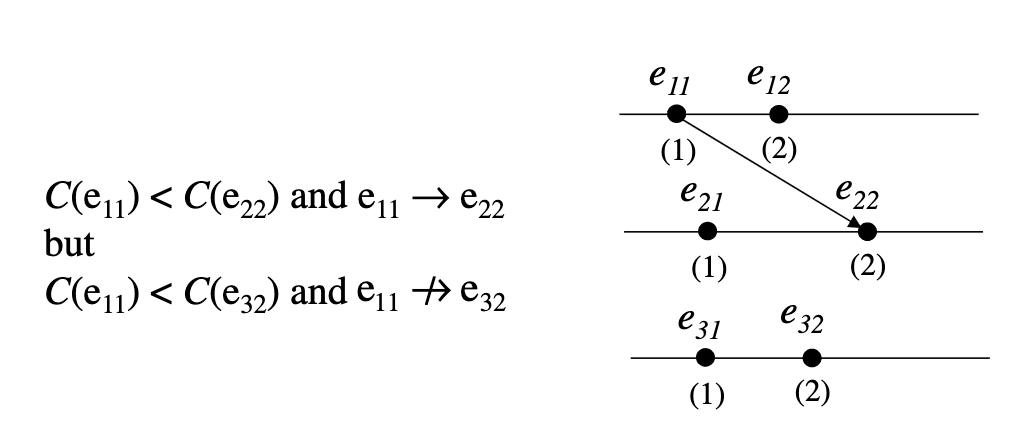
\includegraphics[width=0.3\linewidth]{opposite.png}
          \caption{}
        \end{figure}

  \item Vector Clocks addresses this limitation.
\end{itemize}

\subsection{Vector Clocks}
\begin{figure}[h]
  \centering
  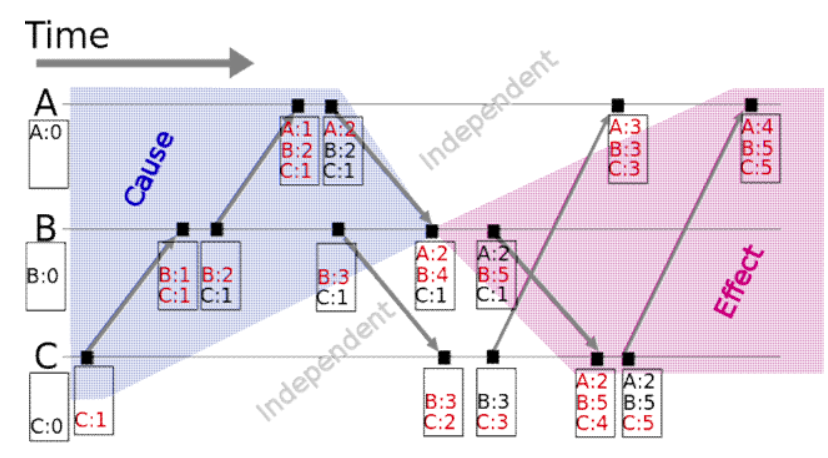
\includegraphics[width=0.5\linewidth]{vec_lock.png}
  \caption{$\mathbf{V}<\mathbf{V}^{\prime}$ if $\leq$ on each element and $<$ on at least one element}
\end{figure}
We have the problem that the system will halt if one process fails. To Generalize, all the workers for any synchronization that can be specified in terms of a State Machine
The main problem in totally ordering events is that two or more events at different processes may have identical timestamp, which can be resolved by identical process id.

In the system of vector clocks, the time domain is represented by a set of $n$-dimensional nonnegative integer vectors. Each process $p_{i}$ maintains a vector $v t_{i}[1 . . n]$, where $v t_{i}[i]$ is the local logical clock of $p_{i}$ and describes the logical time progress at process $p_{i} . v t_{i}[j]$ represents process $p_{i}$ 's latest knowledge of process $p_{j}$ local time. If $v t_{i}[j]=x$, then process $p_{i}$ knows that local time at process $p_{j}$ has progressed till $x$. The entire vector $v t_{i}$ constitutes $p_{i}$ 's view of the global logical time and is used to timestamp events.
Process $p_{i}$ uses the following two rules $R 1$ and $R 2$ to update its clock:

\begin{itemize}
  \item Before executing an event, process $p_{i}$ updates its local logical time $v t_{i}[i]:=v t_{i}[i]+d \quad(d>0)$.
  \item $R 2:$ Each message $m$ is piggybacked with the vector clock $v t$ of the sender process at sending time. On the receipt of such a message $(m, v t)$, process $p_{i}$ executes the following sequence of Update the global logical time $v t_{i}[k]:=\max \left(v t_{i}[k], v t[k]\right)$, executes the first step and deliver the message $m$.
\end{itemize}
\subsubsection{Physical Clocks}
Physical clocks are synchronized to an accurate real-time standard like UTC. Let $C_{i}(t)$ denote the reading of clock $C_{i}$ at physical time $t$. Assume $C_{i}(t)$ is a continuous, differentiable function of $t$, except for isolated jump discontinuities where clock is reset. We have 2 properties:
\begin{itemize}
  \item There exists constant $\kappa \ll 1$ s.t. for all $i:\left|\frac{d C_{i}(t)}{d t}-1\right|<\kappa$
  \item For all $i, j:\left|C_{i}(t)-C_{j}(t)\right|<\epsilon$ for small constant $\epsilon$
\end{itemize}

One distributed implementation can be:
\begin{itemize}
  \item If $P_{i}$ does not receive a message at physical time $t$ then $\frac{d C_{i}(t)}{d t}>0$
  \item $P_{i}$ sends $T_{m}=C_{i}(t)$ along with its message, and upon receiving that message at time $t^{\prime}$,
        $P_{j}$ sets $C_{j}\left(t^{\prime}\right)=\max \left(\lim _{\delta \rightarrow 0} C_{j}\left(t^{\prime}-|\delta|\right), T_{m}+\mu_{m}\right)$
\end{itemize}

\subsection{We can Lamport clocks to achieve mutual exclusion}
With the upper go implementation, we just need to add 2 helper functions:
\begin{lstlisting}
// Check if all *other* processes have advanced to later logical times // Check whether the current process has the lock     
func (state *LamportLockState) allProcessesSeen(time int) bool {       func (state *LamportLockState) haveLock() bool {     
	for p := range state.seen {                                 	// peek at the head of the queue                           
		if p != state.proc {                                  	state.lock.Lock()                       
			if state.seen[p] < time {                     	if state.reqs.Len() > 0 {                             
				return false                      	m := (*state.reqs)[0]        
			}                                   		if m.Proc == state.proc {     
		}                                   			if state.allProcessesSeen(m.Time) {
	}                                  	                    	state.lock.Unlock() 
	return true                        	                    	return true               
}                                                      			}}}
                                                               		state.lock.Unlock()
                                                               		return false}
\end{lstlisting}

In function Acquire(), we just have to check whether it haveLock() to get the lock to prevent another process to enter the mutual exclusion.
\subsection{We can use the physical clock to implement Network Time Protocol}
Assume that clocks $A$ and $B$ are stable and running at the same speed. Let $a=T_{1}-T_{3}$ and $b=T_{2}-T_{4}$. If the network delay difference from $A$ to $B$ and from $B$ to $A$, called differential delay, is small, the clock offset $\theta$ and roundtrip delay $\delta$ of $B$ relative to $A$ at time $T_{4}$ are approximately given by $\theta=\frac{a+b}{2}, \quad \delta=a-b$.
\begin{figure}[h]
  \centering
  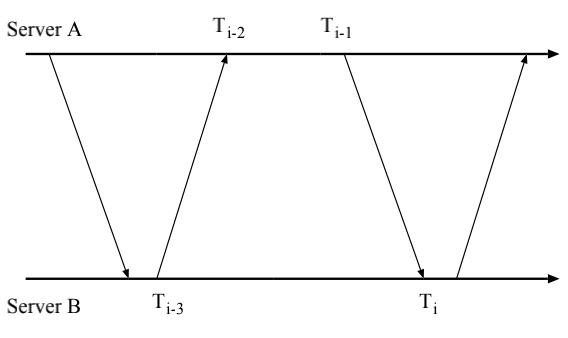
\includegraphics[width=0.3\linewidth]{ntp.png}
  \caption{}
\end{figure}

\section{Weak Point of the paper}
\subsection {No strongly provincial performance tests}
To ensure the partial order, we have multiple implementations based on the condition and the pseudocode. In this paper \cite{fidge1987timestamps},
the author gives a more convincing example with scale time changing at one state machine and provides the testing results for their algorithm.
Based on newly proposed systems like kafka \cite{Bench-kafka} or more recent paper \cite{kshemkalyani2020prime} using vector clock to store timestamp, we knew that the stability of vector clock is really good.
\subsection{Limitations of the proposed clock}
I've discussed the Lamport clock's limitation and vector clock resolves it. As for vector clock, because we obtain the timestamp in random order, we lose the track of timestamp sequence.
\section{Possible Refinement to the idea}
\subsection {More efficient implementation for vector clock}
\subsubsection {Singhal-Kshemkalyani’s Differential Technique}

The observation that between successive message sends to the same process can be optimized by a differential technique:
$p_j$ have the timestamp form of $\left\{\left(i_{1}, v_{1}\right),\left(i_{2}, v_{2}\right), \ldots,\left(i_{n_{1}}, v_{n_{1}}\right)\right\}$.
When $p_j$ receives the message of compressed timestamp, it updates its vector clock with $v t_{i}[k]=\max \left(v t_{i}[k], v_{k}\right)$ for $k=1,2, \ldots, n_{1}$\dots

\subsection {Better implementation for fault tolerance}
In filesystems or databases, we have Redo/Undo Logging or Sharpshooting for fault tolerance. In the paper,
if one process in the distributed system is down, the whole system will crash. In \textit{Parallel Virtual File System} \cite{carns2000pvfs}, those logging techniques are illustrated one by one,
and in \cite{choi2020libnvmmio}, we even could use the hybrid method to utilize the performance of fault tolerance.

\subsection{Another locks for synchronization}
In databases, we have two phase lock to maintain concurrency, basically the write exclusive, read shared lock to maintain the highest qps.
\subsection{Better implementation for NTP protocol}
In High Frequency Trading Firm, we don't use NTP, rather, we use PTP. It is a protocol using hardware to record the tiem
\cite{HFT-PTP-NTP} %beter NTP portocol

Every PTP sequence involves a series of four messages between master and slave:
\begin{itemize}
\item The initial sync message from master to slave
\item A follow-up sync message from master to slave
\item A delay request message from slave to master
\item A final delay response message from master to slave
\end{itemize}


\bibliographystyle{ACM-Reference-Format}
\bibliography{clocks_and_the_ordering_of_events_in_a_distributed_system}

\end{document}
\endinput
%%
%% End of file `sample-acmlarge.tex'.
